% \usepackage[normalem]{ulem}
% \usepackage{array}
% \usepackage{longtable}
% \usepackage{hhline}
% \usepackage{colortbl}

\chapter{Contexte général du projet}
\section*{Introduction}
\addcontentsline{toc}{section}{Introduction}
Dans ce chapitre, nous allons introduire le contexte général du projet réalisé lors de mon stage à HPS. Nous commencerons par présenter l'entreprise HPS, mettant en lumière sa structure, son secteur d'activité et son historique. Cette introduction fournira un aperçu de l'environnement dans lequel le projet s'est déroulé et permettra de mieux comprendre le contexte dans lequel les solutions que nous avons développées ont été mises en œuvre. Nous aborderons ensuite la problématique du projet, qui a guidé notre travail tout au long du stage. Cela comprendra une discussion sur les principaux défis identifiés qui ont motivé la mise en œuvre de ce projet. Enfin, nous décrirons comment le projet a été planifié et conduit durant la période de stage. Cette section fournira des détails sur les différentes phases du projet, les décisions prises et les étapes réalisées tout au long du stage. L'objectif est de donner un aperçu du processus de gestion de projet, depuis la planification jusqu'à la réalisation, en passant par le suivi et le contrôle des différentes tâches. 

Ce chapitre permet de mieux comprendre le contexte et les enjeux du projet, offrant ainsi un fondement pour l'analyse détaillée des travaux effectués durant le stage qui seront présentés dans les chapitres suivants. 

\section{Présentation de l’organisme d’accueil}
\subsection{L’entreprise HPS }
Depuis sa création en 1995, HPS a connu une croissance rapide et s'est positionnée comme l'un des leaders mondiaux dans le secteur des technologies de cartes et de paiements. Avec une présence dans 90 pays et plus de 450 clients, HPS propose des solutions de paiement avancées à ses clients. Sa mission principale a toujours été de fournir des solutions technologiques novatrices couvrant l'ensemble de la chaîne de valeur des paiements. Grâce à son progiciel PowerCARD, HPS permet à ses clients d'innover rapidement et de lancer facilement de nouveaux produits sur le marché. PowerCARD est parfaitement intégré à tous les réseaux de paiement internationaux et offre un support complet des principales fonctions de paiement en back-office \cite{hps-site}.


La figure suivante représente les régions de présence de HPS au monde : 

\begin{figure}[H]
    \centering
     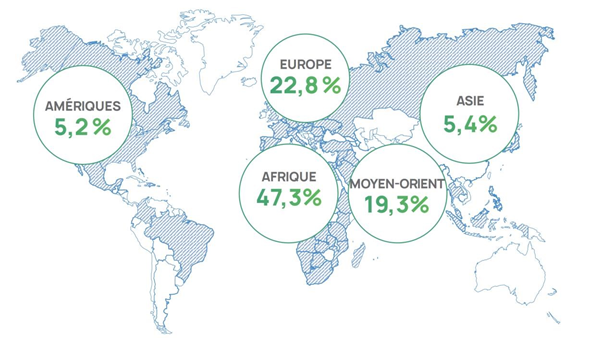
\includegraphics [width=0.7\textwidth]
     {figures/images/Repartition_HPS.png}
    \caption{{Répartition des revenus de HPS par zone géographique}}
    \label{fig:Répartition des revenus de HPS par zone géographique }
\end{figure}

Cette carte illustre la répartition des revenus de HPS par zone géographique. On constate une forte concentration des revenus en Afrique (47,3 \%), suivie de l’Europe (22,8 \%) et du Moyen-Orient (19,3 \%), ce qui témoigne de la position stratégique de HPS sur ces marchés. L’Asie (5,4 \%) et les Amériques (5,2 \%) représentent une part plus modeste, mais traduisent une présence mondiale croissante. Cette répartition reflète la stratégie d’expansion internationale de l’entreprise et sa capacité à s’adapter aux spécificités régionales dans le domaine des paiements électroniques \cite{hps-site}.

\subsection{l'organigramme de l'entreprise d'acceuil}
Depuis sa fondation, la structure organisationnelle de HPS a évolué pour s'ajuster aux exigences du secteur et favoriser une croissance durable. Elle a été soumise à de multiples analyses pour aboutir à une configuration à plusieurs niveaux parallèles, apte à répondre aux besoins variés de tous les domaines d'activité de HPS\cite{hps-site}. 

\begin{figure}[H]
    \centering
     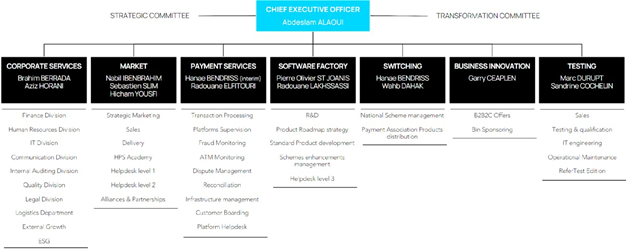
\includegraphics [width=1\textwidth]
     {figures/images/Organigramme_HPS.png}
    \caption{{Organigramme HPS Maroc} \cite{hps-site}}
    \label{fig:Organigramme HPS Maroc}
\end{figure}
\vspace{0.5cm}

Cet organigramme présente la structure organisationnelle actuelle de HPS Maroc, articulée autour du Chief Executive Officer et de plusieurs pôles stratégiques. Chaque pôle  tels que Corporate Services, Market, Payment Services, Software Factory, Switching, Business Innovation ou Testing regroupe des équipes spécialisées en charge de domaines clés comme la recherche et développement, la supervision des transactions, les partenariats, ou encore la qualité logicielle. Cette organisation en silos parallèles permet à HPS de répondre efficacement aux enjeux de performance, d’innovation et de réactivité dans un secteur en constante évolution \cite{hps-site}.

\subsection{Les partenaires de HPS}

HPS a tissé des liens solides avec les acteurs majeurs du marché des cartes en qualité de membre au \textit{Visa Vendor Program}, au \textit{MasterCard Vendor Program}, en tant que partenaire \textit{Oracle}, \textit{Sun Partner Advantage}, \textit{IBM Business Partner} et membre du \textit{IFX Forum}. Cette collaboration étroite s'étend également aux principaux réseaux de paiement internationaux ainsi qu'aux principaux fournisseurs de solutions matérielles et logicielles, d'équipements de paiement et de dispositifs de sécurité \cite{hps-site}.

Par ailleurs, grâce à la polyvalence et à la souplesse du produit \textit{PowerCARD}, HPS propose ses solutions sur les marchés du monde entier, en s'appuyant sur son propre réseau de distribution directe et en partenariat avec des distributeurs de renom.

\begin{figure}[H]
    \centering
     
\includegraphics [width=1\textwidth]
     {figures/images/Partenaires_HPS .png}
    \caption{{Les partenaires de HPS } \cite{hps-site}}
    \label{fig:Les partenaires de HPS}
\end{figure}

La figure ci-dessus regroupe les logos des partenaires stratégiques de HPS, répartis en trois catégories. On y retrouve tout d'abord des intégrateurs technologiques et distributeurs internationaux (ex. : \textit{BFI}, \textit{ObjectWay}, \textit{RAYA}), ensuite des fournisseurs de technologies informatiques majeurs comme \textit{HP}, \textit{IBM} et \textit{Oracle}, et enfin des acteurs de premier plan dans le domaine des réseaux de paiement et de la sécurité, tels que \textit{Visa}, \textit{MasterCard}, \textit{American Express}, \textit{JCB}, \textit{Thales}, \textit{Fujitsu}, \textit{Diebold} et \textit{Safenet}. Ces partenariats renforcent la capacité de HPS à proposer des solutions globales, sécurisées et interopérables à l’échelle internationale \cite{hps-site}.


\subsection{Progiciel PowerCARD}

\begin{figure}[H]
    \centering
    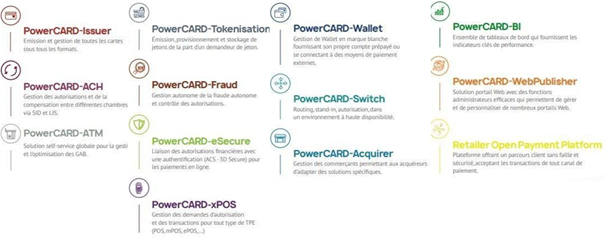
\includegraphics[width=0.9\textwidth]{figures/images/Solutions_PowerCARD .png}
    \caption{Suite de Solutions PowerCARD \cite{hps-site}}
    \label{fig:solutions-powercard}
\end{figure}

La plateforme \textit{PowerCARD} est la suite de solutions de paiement électronique développée par le Groupe HPS. Elle se démarque par sa sécurité, sa fluidité et la robustesse de son traitement des flux d’informations et des transactions. Elle offre également une expertise à toutes les étapes du cycle des opérations de paiement. Les utilisateurs des solutions \textit{PowerCARD} bénéficient d’une expérience de paiement fluide et multicanale, tandis que les opérateurs peuvent maîtriser leurs coûts de traitement des transactions et assurer une remontée d’information à forte valeur ajoutée.

Au fil des années, HPS a construit une véritable communauté à l’échelle internationale, composée d’utilisateurs et d’experts de l’industrie du paiement, qui se réunissent régulièrement à l’occasion du \textit{PowerCARD Users Meeting} dans le but de discuter des dernières évolutions du secteur et de faire évoluer les pratiques et les solutions de paiement sur le plan international \cite{hps-site}.

\subsection{HPS Switch}

\paragraph{}
HPS intervient également au niveau national à travers \textbf{HPS Switch}, une plateforme dédiée à la gestion des transactions monétiques et mobiles. Ce service assure le routage, la compensation et le règlement des paiements électroniques, permettant aux différents acteurs du secteur financier marocain de s’interconnecter de manière sécurisée.Il s’agit d’un maillon essentiel de l’écosystème monétique national, garantissant
l’interopérabilité entre les banques, les établissements de paiement et les réseaux de cartes.\textbf{HPS Switch} contribue ainsi à la fiabilité des échanges financiers tout en respectant les exigences réglementaires fixées par \textit{Bank Al Maghrib} \cite{hps-site}.

\begin{figure}[H]
    \centering
    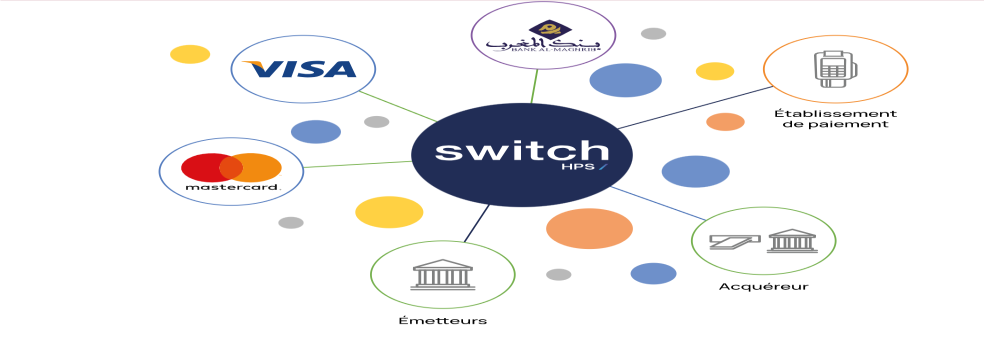
\includegraphics[width=0.9\textwidth]{figures/images/Switch.png}
    \caption{Switch \cite{hps-site}}
    \label{fig:solutions-powercard}
\end{figure}





\section{Présentation du projet}
\subsection{Contexte du projet}

Dans le domaine des transactions financières électroniques, le protocole \textbf{ISO 8583} est aujourd’hui devenu la norme incontournable dans les systèmes de paiement électronique pour l’échange de messages entre les (\textit{DAB}), les terminaux de paiement, les serveurs bancaires et les réseaux interbancaires. Il permet de structurer des messages complexes à caractère transactionnel (autorisations, retraits, paiements, etc.).Cependant, les systèmes actuels utilisant ce protocole évoluent généralement dans des environnements fermés, critiques et strictement réglementés, rendant leur accès difficile, voire impossible, pour les développeurs, les testeurs ou les stagiaires souhaitant travailler sur des tâches liées à la simulation ou à l’intégration. Cela complique considérablement la compréhension, le test et la validation des mécanismes d’échange ISO en conditions réelles.Face à ces difficultés, la mise en place d’un simulateur \textbf{ISO 8583} autonome, flexible et didactique s’impose comme une nécessité. Un tel outil offrirait la possibilité de générer, envoyer, recevoir et analyser des messages ISO de manière totalement indépendante, sans recourir à une infrastructure bancaire réelle.Il permettrait également la définition de multiples scénarios de test (transactions réussies, erreurs, délais, interruptions) tout en garantissant un suivi centralisé et transparent des \textit{logs}. Une solution de ce type favoriserait non seulement l’apprentissage technique du protocole \textbf{ISO 8583}, mais aussi la validation fonctionnelle et l’intégration continue de modules monétiques dans des environnements modernes, sécurisés et maîtrisés.


\subsection{Problématique}

À l’ère du numérique, les transactions financières électroniques telles que les paiements par carte bancaire, les retraits aux distributeurs (DAB), ou encore les virements sont devenus omniprésentes et essentielles au bon fonctionnement de l’économie. Ces échanges doivent respecter des normes strictes afin de garantir la \textbf{sécurité}, la \textbf{fiabilité}, l’\textbf{interopérabilité} et la \textbf{rapidité} des opérations.
L’un des protocoles les plus utilisés dans ce domaine est \textbf{l’ISO 8583}, un standard international permettant d’échanger des messages entre les différents composants du système de paiement (terminaux de paiement, serveurs bancaires, passerelles de paiement, etc.). Toutefois, \textbf{sa structure est complexe}, souvent binaire ou encodée de façon rigide, ce qui rend sa manipulation, son décodage et son interprétation particulièrement \textit{délicats}.
Dans ce contexte, les entreprises comme \textbf{HPS}, qui fournissent des solutions de paiement, doivent impérativement tester et valider ces échanges avant leur mise en production. Mais cette phase de test soulève plusieurs problématiques majeures :

\begin{itemize}
    [label=\textbullet] \item \textbf{Accès limité aux environnements bancaires réels} : les environnements de production sont souvent protégés et coûteux à utiliser pour des tests.
    \vspace{0.5cm}

    \item \textbf{Coût élevé des outils de simulation du marché} : les simulateurs existants sont généralement propriétaires, chers, et peu flexibles.
    \vspace{0.5cm}

    \item \textbf{Difficulté à reproduire des scénarios variés} : il est compliqué de tester des cas comme les refus de transaction, les erreurs réseau, les réponses tardives, ou les pertes de connectivité.
    \vspace{0.5cm}

    \item \textbf{Complexité technique des messages ISO 8583} : le codage/décodage des trames nécessite une expertise spécifique et ralentit les phases de développement et de \textit{debug}.
    \vspace{0.5cm}

    \item \textbf{Absence de centralisation des logs et monitoring} : il est difficile d'analyser en temps réel les messages échangés, ce qui nuit à la détection rapide des anomalies.
\end{itemize}
Ces défis freinent la productivité des équipes techniques (développeurs, testeurs, support), rallongent les cycles de développement et exposent l’entreprise à des risques en cas de dysfonctionnements non détectés avant le déploiement.C’est donc pour répondre à ces limitations qu’un \textbf{simulateur ISO 8583 interne}, basé sur une architecture \textit{microservices}, devient une \textbf{solution stratégique}. Il permettra de :

\begin{itemize}
     [label=\textbullet]\item \textbf {Automatiser et fiabiliser les tests}.
     \vspace{0.5cm}
    \item \textbf {Reproduire une grande variété de scénarios réalistes}.
    \vspace{0.5cm}
    \item \textbf {Gagner en réactivité lors de la validation ou du support}.
    \vspace{0.5cm}
    \item \textbf {Offrir une base flexible et évolutive pour de futurs projets d’innovation}.
\end{itemize}




\subsection{Objectif}

Le projet consiste à concevoir et développer une plateforme configurable de test de performance et de montée en charge pour les messages \textbf{ISO 8583}, reposant sur une architecture \textit{microservices}. Cette plateforme a pour but de simuler les interactions réalisées par les canaux de paiement électroniques, notamment entre les  (\textit{POS}), les (\textit{ATM}) et les systèmes internes bancaires via le réseau de messagerie financière.

Le simulateur devra être capable d’émuler fidèlement le comportement de ces systèmes tout en permettant des tests intensifs, sûrs et flexibles. Il intégrera ainsi plusieurs fonctionnalités clés, notamment :

\begin{itemize}[label=\textbullet]
     \item \textbf{Validation des champs ISO 8583 et construction dynamique des messages.}
       \vspace{0.5cm}
    \item \textbf{Chiffrement et déchiffrement des données sensibles selon les normes de sécurité.}
      \vspace{0.5cm}
    \item \textbf{Vérification des messages entrants et génération automatique des réponses ISO 8583.}
      \vspace{0.5cm}
    \item \textbf{Gestion de la communication synchrone entre les microservices du simulateur.}
      \vspace{0.5cm}
    \item \textbf{Analyse des journaux (logs) pour permettre un suivi, un débogage et une évaluation des tests en temps réel.}
\end{itemize}


\subsection{Périmètre du projet}

Afin de cadrer précisément la problématique et les objectifs du projet, une analyse fondée sur la méthode \textbf{QQOQCP} a été menée. Cette approche a permis d’identifier les éléments clés en interaction et de structurer de manière cohérente les besoins fonctionnels et techniques.

\begin{table}[H]
\centering
\rowcolors{2}{blue!10!white}{white}
\renewcommand{\arraystretch}{1.5}
\begin{tabular}{|>{\bfseries}c|m{4cm}|m{7cm}|}
\hline
\rowcolor{blue!20}
\textbf{Question} & \textbf{Élément} & \textbf{Réponse} \\
\hline
\textbf{Qui?} & Utilisateurs cibles & Développeurs, testeurs, administrateurs système et équipes qualité travaillant sur les systèmes de paiement électronique utilisant le standard ISO 8583. \\
\hline
\textbf{Quoi?} & Objectif du projet & Développement d'une plateforme de simulation ISO 8583 basée sur une architecture microservices permettant de générer, valider, tracer et analyser les transactions financières. \\
\hline
\textbf{Où?} & Contexte d'utilisation & Besoin d'un outil automatisé, flexible et sécurisé pour tester les messages ISO 8583, remplaçant les méthodes manuelles moins efficaces ou les outils internes obsolètes. \\
\hline
\textbf{Quand?} & Période de réalisation & Le besoin de ce projet est apparu avec l'évolution des systèmes de paiement et la nécessité croissante de tester efficacement les échanges entre différents modules (ATM, terminaux POS, commutateurs réseau). \\
\hline
\textbf{Comment?} & Méthode de réalisation & L'application est développée en utilisant une architecture microservices avec Spring Boot, MySQL, Eureka Server et Spring Cloud Gateway. Interface web Angular avec communication HTTP REST (FeignClient), fonctionnalités de packing/unpacking ISO, validation métier, génération PDF, système de logs et alertes email. \\
\hline
\textbf{Pourquoi?} & Justification & Garantir la qualité et la conformité des transactions ISO 8583, améliorer la traçabilité, automatiser les tests et fournir une interface ergonomique pour les utilisateurs techniques et fonctionnels. \\
\hline
\end{tabular}
\caption{Analyse du périmètre du projet HPS selon la méthode QQOQCP}
\label{tab:qqoqcp-hps}
\end{table}








\subsection{Avantages et Bénéfices}

Ce projet apporte une solution efficace pour simuler et analyser les échanges entre les systèmes de paiement. Il permet de tester différents scénarios de transaction de manière sécurisée, rapide et autonome. Grâce à son interface claire et intuitive, il facilite la compréhension des flux d'échange dans les environnements bancaires. C'est un outil précieux pour la formation, le développement, et l'amélioration continue des systèmes financiers, tout en réduisant les risques d'erreurs lors de la mise en production.

L'architecture microservices adoptée offre une flexibilité et une scalabilité remarquables, permettant une maintenance simplifiée et des mises à jour sans interruption de service. La conformité au protocole ISO8583 garantit l'interopérabilité avec les systèmes bancaires existants et assure la compatibilité avec les standards internationaux. De plus, le système de monitoring intégré et la gestion des incidents permettent une surveillance proactive et une résolution rapide des problèmes, contribuant ainsi à la fiabilité et à la performance globale du simulateur.



\section{Méthodologie de travail }
\subsection{L’approche Agile}

Les méthodes \textit{agiles} (ou \textit{"agile methodologies"} en anglais) regroupent différentes approches de gestion de projet qui mettent l'accent sur la flexibilité, l'adaptabilité et la réactivité face aux changements. Les approches agiles permettent de s'adapter rapidement aux changements de priorités, aux nouveaux besoins des clients ou aux conditions du marché.Cela est particulièrement important dans les environnements en constante évolution, où les exigences ne sont pas toujours clairement définies au départ. Ainsi, elles favorisent une collaboration étroite entre les équipes de développement, les clients et les parties prenantes.La méthodologie Agile se base sur ce principe simple : \og planifier la totalité de votre projet dans les moindres détails avant de le développer est contre-productif \fg. En effet, la méthode Agile recommande de se fixer des objectifs à court terme. Le projet est donc divisé en plusieurs sous-projets. Une fois l’objectif atteint, on passe au suivant jusqu’à l’accomplissement de l’objectif final. 

Autre point important : la méthode Agile repose sur une relation privilégiée entre le client et l’équipe projet, la satisfaction du client étant la priorité.L’approche Agile offre une plus grande flexibilité et une meilleure visibilité dans la gestion du projet. À notre époque où la personnalisation est si importante, cette méthodologie fait de plus en plus d’adeptes \cite{agile-manifesto}.


\subsection{Méthodologie Scrum}

La méthode \textbf{Agile Scrum} est une méthodologie de gestion de projet. C’est certainement la plus utilisée et la plus connue, puisqu’elle est cohérente avec la réalité de la réalisation des projets informatiques tels qu’ils sont aujourd’hui. Elle est également très intuitive, facile à comprendre et à implémenter.
La méthode \textit{Scrum} fait partie des méthodologies de la famille \textit{Agile}. L’approche agile consiste à se donner des objectifs à court terme. Une fois un objectif terminé, on fait le point, puis on fixe un nouvel objectif en fonction des résultats obtenus, et ainsi de suite jusqu’à atteindre le résultat final.
Le commanditaire est impliqué dans le projet du début à la fin, ce qui lui donne de la visibilité. Cela permet notamment d’éviter l’\textbf{effet tunnel} : se lancer dans un projet et arriver à terme avec un produit qui ne correspond pas aux attentes du client, ou ne pas pouvoir mener le projet à son terme \cite{scrum-guide}.


\begin{figure}[H]
    \centering
     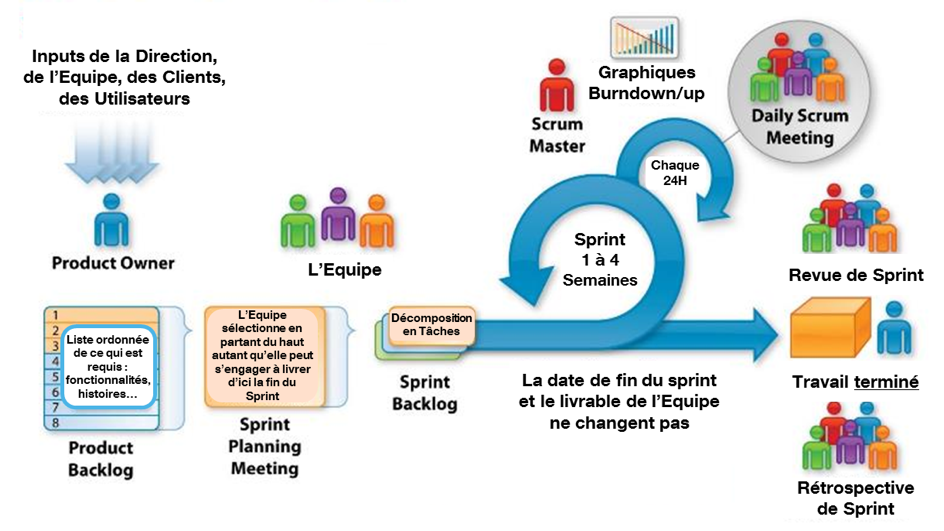
\includegraphics [width=1\textwidth]
     {figures/images/Process-AGILE.png}
    \caption{{Processus Scrum} \cite{scrum-guide}}
    \label{fig:Diagramme de Gantt}
\end{figure}

Cette image illustre le processus de développement selon la méthode \textbf{Scrum}, une approche Agile centrée sur l’itération continue et l’implication du client. Le cycle commence par le \textit{Product Owner}, qui établit une liste priorisée des fonctionnalités à développer appelée \textit{Product Backlog}. Lors du \textit{Sprint Planning Meeting}, l’équipe sélectionne les éléments qu’elle s’engage à réaliser dans un \textit{Sprint}, une période de 1 à 4 semaines.Les éléments sélectionnés sont transférés dans le \textit{Sprint Backlog}, puis décomposés en tâches. Durant le Sprint, des réunions quotidiennes (\textit{Daily Scrum Meetings}) sont organisées pour assurer le suivi et ajuster les efforts. Le \textit{Scrum Master} accompagne l’équipe pour lever les obstacles et suivre l'avancement à l’aide de graphiques (ex. : burndown chart).

À la fin du Sprint, une \textit{Revue de Sprint} est organisée pour présenter les livrables, suivie d’une \textit{Rétrospective de Sprint} qui permet à l’équipe d’identifier des axes d’amélioration. Ce processus cyclique vise à livrer un produit fonctionnel à chaque itération, en impliquant continuellement les parties prenantes.

\subsection{Equipe Scrum }


L'équipe Scrum est composée de trois rôles clés, chacun exerçant des responsabilités bien définies :

\begin{itemize}
    [label=\textbullet] \item \textbf{Scrum Master} : il est, en quelque sorte, le coach de l’équipe. C’est lui qui a pour mission de tirer le meilleur de chaque membre de l’équipe afin de faire avancer efficacement le projet et de garantir la satisfaction client. Il est notamment le garant de la bonne compréhension de la méthodologie de projet agile par l’ensemble de l’équipe. Il est, par ailleurs, le responsable du planning des sprints, des \textit{Daily} (réunions quotidiennes appelées \textit{mêlées}) et des \textit{Sprint Reviews}.
     \vspace{0.5cm}

    \item \textbf{Product Owner} : aussi appelé chef de projet digital, le Product Owner est le garant du respect et de la satisfaction client. Il est à la fois chargé de définir et garantir la vision produit, mais également d’alimenter le \textit{Product Backlog}.
     \vspace{0.5cm}

    \item \textbf{Équipe de développement} : l’équipe de développement est chargée de transformer les besoins définis par le Product Owner en fonctionnalités utilisables. Pluridisciplinaire, elle possède en interne toutes les compétences nécessaires à la réalisation du projet. La taille idéale de l’équipe de développement est comprise entre 2 et 5 personnes. La notion de hiérarchie est absente, les décisions sont prises collégialement \cite{scrum-guide}.
     \vspace{0.5cm}
\end{itemize}




\subsection{Planification des Sprints}

Nous avons planifié des sprints d’une durée variant de une à deux semaines, en fonction de la complexité des tâches à réaliser et de la disponibilité de l’équipe.

Chaque sprint débute par une réunion de planification, au cours de laquelle l’ensemble de l’équipe se réunit pour :
\begin{itemize} [label=\textbullet]
    \item Définir les objectifs du sprint à venir ;
    \item Identifier et prioriser les tâches à accomplir ;
    \item Estimer la charge de travail pour chaque tâche ;
    \item Attribuer les tâches aux différents membres de l’équipe, en tenant compte de leurs compétences et de leur charge actuelle.
\end{itemize}

Cette organisation permet d’assurer une répartition équilibrée du travail, de clarifier les attentes pour chaque membre et de garantir que les objectifs du sprint soient atteints dans les délais impartis.

À la fin de chaque sprint, une réunion de revue est organisée afin d’évaluer l’avancement, de présenter les fonctionnalités développées et d’identifier les points d’amélioration pour les sprints suivants.


\subsection{Identification des sprints}
L’identification des sprints consiste à prévoir les missions du projet tout au long des phases consistant le cycle de développement.

\begin{table}[H]
\centering
\rowcolors{2}{blue!10!white}{white}
\renewcommand{\arraystretch}{1.5}
\begin{tabular}{|>{\bfseries}c|m{4cm}|m{9cm}|}
\hline
\rowcolor{blue!20}
Sprint & \textbf{Titre du sprint} & \textbf{Objectif principal} \\
\hline
Sprint 1 & Mise en place de l'infrastructure & \textbf{Créer} la structure du projet avec \texttt{GatewayService}, Eureka, et \textbf{développer} \texttt{AuthService} avec JWT. \\
\hline
Sprint 2 & Service de génération ISO & \textbf{Développer} \texttt{PackingISOService} pour la génération de messages ISO 8583 avec les 49 champs. \\
\hline
Sprint 3 & Service de dépaquetage ISO & \textbf{Développer} \texttt{DepackingISOService} pour l'analyse et la décomposition des messages ISO. \\
\hline
Sprint 4 & Service de traitement des réponses & \textbf{Développer} \texttt{ResponseISOService} pour la réception et le traitement des réponses ISO. \\
\hline
Sprint 5 & Service d'historique des transactions & \textbf{Développer} \texttt{TransactionHistoryService} pour l'enregistrement et la consultation de l'historique. \\
\hline
Sprint 6 & Service de gestion des incidents & \textbf{Développer} \texttt{IncidentReportService} pour la déclaration et le suivi des incidents. \\
\hline
Sprint 7 & Service de monitoring et logs & \textbf{Développer} \texttt{MonitoringService} pour la surveillance des logs système. \\
\hline
Sprint 8 & Service de gestion des comptes et cartes & \textbf{Développer} \texttt{AccountCardService} pour la gestion des comptes bancaires et des cartes. \\
\hline
Sprint 9 & Interface utilisateur - Authentification & \textbf{Développer} l'interface Angular pour l'authentification et la gestion des rôles. \\
\hline
Sprint 10 & Interface utilisateur - Administrateur & \textbf{Développer} les interfaces Angular pour l'administrateur : génération et dépaquetage des messages ISO, gestion des comptes et cartes. \\
\hline
Sprint 11 & Interface utilisateur - Testeur & \textbf{Développer} les interfaces Angular pour le testeur. \\
\hline
\end{tabular}
\caption{Liste détaillée des sprints du projet}
\label{tab:sprints-projet}
\end{table}


\subsection{Choix de la méthode Agile Scrum}

Nous avons choisi la méthode \textbf{Agile Scrum} pour plusieurs raisons importantes :

\begin{itemize} [label=\textbullet]
    \item \textbf{Flexibilité et Adaptabilité} : Scrum nous permet d'ajuster nos plans et nos priorités en fonction des besoins qui évoluent, ce qui est fréquent dans le développement de logiciels.
    
    \item \textbf{Travail d'Équipe et Communication} : Scrum encourage une collaboration étroite entre les membres de l'équipe et les parties prenantes, ce qui facilite la communication et la résolution rapide des problèmes.
    
    \item \textbf{Livraisons Fréquentes} : Grâce aux itérations courtes, Scrum nous permet de livrer des fonctionnalités rapidement, d'obtenir des retours plus tôt et de nous assurer que le projet évolue dans la bonne direction.
    
    \item \textbf{Transparence} : Scrum favorise la transparence à travers des réunions régulières (\textit{Daily Meetings}, \textit{Sprint Reviews}) et une documentation continue, ce qui évite les surprises.
    
    \item \textbf{Amélioration Continue} : Chaque sprint se termine par une rétrospective permettant d'analyser ce qui a bien fonctionné et ce qui doit être amélioré, afin d'optimiser la productivité et la qualité du projet.
    
    \item \textbf{Équipe Engagée} : Scrum responsabilise chaque membre de l'équipe en lui donnant un rôle actif dans le projet, ce qui augmente la motivation et l'efficacité globale.
\end{itemize}

En choisissant Scrum, nous visons à rendre notre projet plus flexible, collaboratif et à livrer une solution répondant aux besoins en constante évolution de nos utilisateurs.

\medskip
En résumé, la méthode \textbf{Agile}, et plus particulièrement \textbf{Scrum}, a été choisie pour ses avantages tels que l'adaptabilité, la collaboration, les livraisons itératives, la transparence, la gestion itérative et l'engagement de l'équipe. Contrairement aux approches classiques, l'Agile se concentre sur l'évolution progressive du projet en créant des éléments fonctionnels à chaque étape, favorisant ainsi l'ajustement continu et la réalisation des objectifs.









\section{Planification et démarche du projet}

\subsection{Planification}

Pour atteindre l’objectif fixé, la planification est une phase indispensable. Sans planification, aucune maîtrise n’est possible et les membres de l’équipe navigueraient à vue. En effet, planifier permet d’organiser le déroulement des étapes du projet dans le temps — une tâche essentielle pour respecter les délais.

Planifier un projet consiste à le découper en plusieurs étapes (identification de l’ensemble des tâches à réaliser), à en estimer la durée, à identifier l’enchaînement logique des étapes (y compris celles pouvant être menées en parallèle : ordonnancement des tâches, chemin critique), à affecter les ressources nécessaires (financières et humaines), puis à modéliser cette organisation à l’aide d’un document opérationnel partagé avec tous les acteurs concernés, afin d’optimiser le déroulement et le suivi du projet.

Dans le cadre de mon projet, les différentes phases et tâches ont été planifiées et classées dans la figure suivante :

\begin{figure}[H]
    \centering
    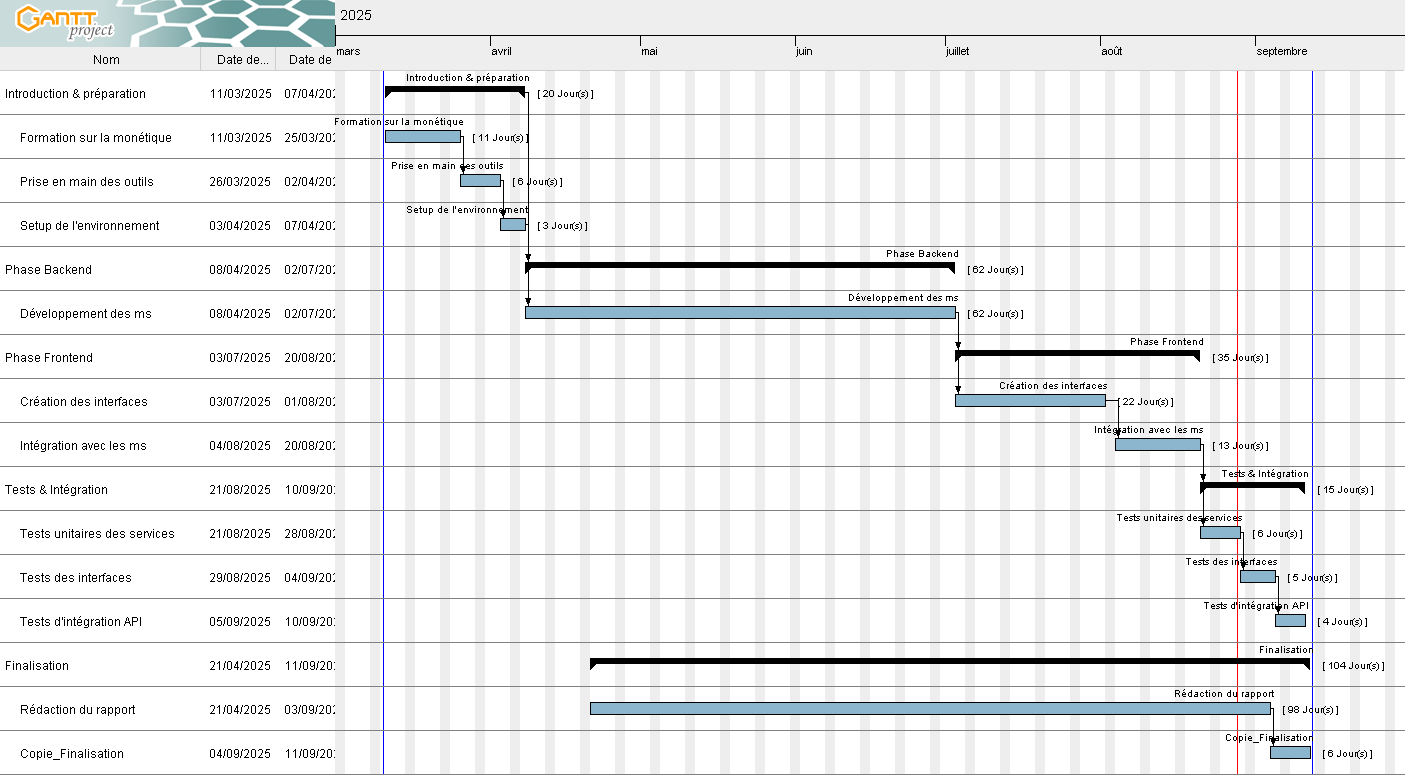
\includegraphics[width=0.98\textwidth]{figures/images/SimulateurGantt.png}
    \caption{Diagramme de Gantt}
    \label{fig:solutions-powercard}
\end{figure}

Pour la réalisation de ce projet, plusieurs étapes ont été planifiées et exécutées, conformément au diagramme de Gantt présenté. Ces étapes sont les suivantes :

\begin{itemize}[label=\textbullet]
    \item \textbf{Phase d’introduction et préparation :} Cette phase a permis de prendre connaissance du contexte général, des attentes du stage, ainsi que des outils et environnements de travail. Elle a également inclus une formation sur les normes et protocoles utilisés dans le projet.      
    \vspace{0.5cm}


    \item \textbf{Analyse et cadrage du projet :} Cette étape a consisté à étudier en profondeur le protocole ISO 8583, à identifier les besoins fonctionnels et non fonctionnels, à définir les spécifications techniques ainsi que l’architecture logicielle à adopter. Elle a abouti à la rédaction du backlog initial.
     \vspace{0.5cm}


    \item \textbf{Conception et développement des services :} Cette phase inclut la planification et le développement des différents microservices du projet (Packing, Transaction, Response, Auth, etc.). Chaque sprint a ciblé un ensemble cohérent de fonctionnalités à implémenter.
     \vspace{0.5cm}


    \item \textbf{Création de l'interface utilisateur :} L’interface front-end a été développée à l’aide d’Angular, permettant à l’utilisateur d’interagir avec les microservices via une interface claire et intuitive. Cette phase a été suivie par le déploiement avec Docker et Kubernetes.
    \vspace{0.5cm}


    \item \textbf{Tests et intégration continue :} Une série de tests unitaires, d’intégration, et fonctionnels ont été réalisés pour valider le bon fonctionnement du système global. L’intégration des microservices et leur communication via Eureka et Gateway ont été vérifiées.
    \vspace{0.5cm}


    \item \textbf{Finalisation et documentation :} Une fois toutes les fonctionnalités implémentées et testées, un rapport de stage a été rédigé. Cette phase inclut également la rédaction technique et la documentation de l’architecture mise en place.
\end{itemize}


%%%
%%%






%%%
%%%

\section*{Conclusion }
\addcontentsline{toc}{section}{Conclusion}
Ce chapitre a permis de présenter l’entreprise HPS, le contexte du projet ainsi que les enjeux liés aux tests des transactions \textbf{ISO 8583}. Face à la complexité et aux contraintes des environnements réels, le développement d’un simulateur interne basé sur une architecture \textit{microservices} s’est imposé comme une solution pertinente. L’approche \textit{Agile}, et plus précisément le cadre méthodologique \textit{Scrum}, a été adoptée afin d’assurer une gestion de projet flexible, collaborative et itérative. Le chapitre suivant sera consacré à la conception fonctionnelle et technique du simulateur.


